\documentclass[../main.tex]{subfiles}
\graphicspath{{\subfix{../images/}}}
\begin{document}
	
\chapter{Discussion and conclusions}
In this chapter the results and conclusions will be presented. At first, the work is summarized. A discussion of the consequences and applications of the results and findings to future work follows, both relating to the STEP mission and future space missions. The latter will be achieved through a discussion of how the findings relate to prior missions such as Kepler and others. Lastly, practical recommendations will be given, and a conclusion will be drawn.


\section{Summary}
This study focused on part of the payload of the proposed astronomical space mission STEP. This is a CCD detector to perform photometric measurements of stars. The mission goals and objectives studied in this work are the detection of exoplanets and measurements of their size. STEP is expected to acquire time-series photometric observations of stars in the near UV and visible light range. Mission requirements presented in this work are based on the findings of the Kepler mission and were explained in section \ref{sec:intromissionreqspecification}. The first requirement is an allowable flux change of $10^{-4}$ due to movements on the CCD plane. The second is measurement of the nonlinearity curve to a precision of at least $5*10^{-4}$.

The main goal of this work was to establish technical hardware requirements related to the payload, from the mission requirements that arise from mission objectives. These are an investigation into the photometric precision obtained from the proposed testing procedure, as well as direct attitude requirements that arise from restrictions on the allowable flux change resulting from attitude errors during observations. The results of these analyses were explained in sections \ref{sec:firstreq} and \ref{sec:secondreq}.

Knowledge of the physical effects and processes of the CCD is important and lead to the development of a characterization procedure found in section \ref{sec:charmeasplan}. These effects are described in chapter \ref{chap:theory}. Based on this knowledge, various correction procedures have been presented. These are the bias, flat-field, and hot pixel corrections. These corrections are applied at the image level. These correction procedures, and how to apply them were discussed in the text above in section \ref{sect:cal}. 

In addition, and most importantly, a calibration of the detector linearity was constructed (see \ref{sect:cal}). It was found that for the Atik 414EX detector, the requirements on the photometric precision could be met. This was explained in more detail in section \ref{sec:firstreq}. \\ 
A measurement procedure that will adequately characterize the noise levels, both photonic-, thermal- and readout noise has been developed and presented in section \ref{sec:attmeasplan}. Knowledge of the first and last are crucial in the experimental procedure to determine the pointing accuracy, where they must account for thetotal noise budget. Relative photonic noise can be reduced by increasing the number of detections made within an image, either by increasing exposure times or observing brighter objects. It is hence dependent on the size of the telescope. 

A white noise source originating from the random fluctuating motion of the satellite is jitter. We should ensure that our signal is dominated by photonic noise and not jitter. This is because thermal noise and readout noise can not be eliminated. The former can be reduced by cooling, but the latter remains constant. Jitter can not be eliminated in practice, and any signal quality gains achieved from reducing the photonic noise below the level of jitter will be in vain. In other words, it is a waste of money if optics are chosen to be better than this level. 

Lastly, an experimental test procedure simulating stellar photometry was developed, to study the effects on the differential flux levels, due to the movement of light centroids on the chip. This outputs a technical attitude requirement related to the ADCS system. These results are tabulated in section \ref{sec:attresults}.

\section{Consequences}
In this section, consequences that arise from the results found above, and their relation to the space mission at hand will be discussed in turn.

\subsection{Measurement of detector linearity}
The linearity curve was measured using a simple setup as described in section \ref{sec:setup} (see figure \ref{fig:setup} in that section). In this setup, a fluorescent light bulb in the ceiling was used, reflected off a white lacquered wooden screen. The detector was pointed into this screen. 

The intensity of the light source was found to vary with time (cf. figures \ref{fig:lightsourcestability1to10}, \ref{fig:lightsourcestability20to100} and \ref{fig:lightsourcestability101to110} in section \ref{sec:stabillitylight}). This temporal variation is of the order of a few percent. This variation did not impact the measurement of the linearity curve, since the effect, under the assumption that the variation is linear between any two data points, may be corrected as described in section \ref{sec:stabillitylight}, using equation \ref{eq:fluxcorrect_timecal}. A reference exposure time is chosen, and this level is remeasured both before and after acquisition of a data point of interest. The mean drift in intensity may then be calculated from these two reference values as described above.

In addition, the precision of the measurement of this curve may be arbitrarily small as it only depends on the number of repeats of the experiment. Errors in the linearity curve prove to be small for even a small number of repeats ($N=10$ was used here). The test procedure detector was able to reach the desired precision within the linear range of the nonlinearity curve, and thus satisfies mission requirements. For redundancy, in this case, the experiment could have been performed using $N=100$ repeats, which was done the first time for this detector. 

These considerations lead to two important conclusions. The first is that the measurement of the linearity of the detector may be performed using simple, inexpensive equipment. It is hence practically feasible to always perform such an experiment before launching the payload in question into space, and the constraining factor is the time available to perform such measurements. There is no need for highly calibrated light sources that don't drift or vary in intensity. As was shown by the above experiments, it may vary a lot. There is also no need to collimate the light source or ensure uniform illumination. 

In this work, reflection off a white lacquered surface was sufficient. Ordinarily, linearity calibrations are performed with expensive, highly calibrated equipment and calibrated integrated light sources. The work in question is a proof of concept that such measures are not necessary. One can argue that the demonstration given here,  using poor light sources, is more useful, as it applies to a more general set of light sources. 

There are two subconclusions to be drawn here. The first is that we can repeat the test in space once the payload is in orbit. We simply need to point the telescope at a \textit{relatively} flat field and acquire the necessary frames to measure the curve. We must also take care not to choose a light source that is too bright, such that we are too reliant on a precise calibration of the exposure time. One such light source could be the moon. The moon is significantly dimmer than Earth, as seen from orbit, while at the same time being a very stable light source in comparison to that of the experimental procedure demonstrated above.
We may then recalibrate, or verify the linearity characterization in space. We may perform the entire set of observations as soon as the spacecraft has reached the desired orbit, to check if the instrument has changed characteristics during the launch phase. At a later time, we can continually measure and track changes in the linearity of the instrument, which may change over time. Since the linearity curve will be known to the desired precision before launching the payload into orbit, it is not necessary to redo the entire experiment. It will be sufficient to test a single data point on the linearity curve. This ensures that it lies within the accepted range of deviation from the original curve. It will also ensure that it has not deviated from the curve measured on the ground. Such tests could be repeated every few days, to keep track of any changes in the linearity of the detector over time. 

The second subconclusion is that virtually anyone may calibrate their arbitrarily chosen equipment. The above experimental procedure is very general and is independent of the choice of detector \textit{and} light source. It is only required that a certain measurement protocol be followed. This means that any CCD detector may be characterized using the above characterization procedure. If budget constraints detector choice, however, the necessary precision may be achieved with enough measurements. Thus, given adequate time, we are not dependent on the trading of this particular scientific requirement. 

The arbitrarily chosen photometric precision may be met in any case. In the spirit of the small satellite revolution, photometric measurements are henceforth even more accessible. Smaller student satellite projects may carry camera payloads that are thoroughly characterized, without great investments in calibration setups and equipment. This result is important. 

One such satellite mission is Danish student satellite mission DISCO-2, which aims to study climate change via earth observations of Greenland. If DISCO-2 is to study changes in the albedo of the ice cap, as a quantitative measure of the recession of the inland ice, linearity must be calibrated. Such a measurement is akin to that of the photometry of a transit described above, where differential flux measurements are predicated on knowledge of the nonlinearity curve.

For larger satellite missions such as the upcoming ESA mission \textbf{PLA}netary \textbf{T}ransits and \textbf{O}scillations of stars (\textbf{PLATO}), there is hardly a good argument for not performing this type of calibration.

\subsection{Testing of pointing stability requirements}
The mission requirements were deduced from the findings of the Kepler mission. These specify that the allowable change in the differential photometric measurement is $0.01\%$.

An experiment to simulate differential photometric measurements of two stars was designed. Time-series data were acquired, allowing small fluctuations in the positions of the light centroids. A drift was observed in the differential flux. This appeared to be correlated with the movement of the light centroid on the chip. To establish if this was a true relationship,  readout- and photonic noise contributions were accounted for. The light source used in the experimental setup was again a fluorescent bulb, and the light spots were arbitrarily defocused on the chip face. The light source intensity, which again is not expected to be stable over longer periods of time, is not an issue as we are dealing with the relative (differential) flux, and any changes in the light source intensity will be common in both of the stars. 

The experiment procedure assumes a simple setup and is easily reproducible. Necessary components are a source to produce two spots of light, and some form of a component to allow movements of the light centroids on the chip. The former may be constructed from cardboard and a piece of tin foil. The latter was achieved by using a simple tip-tilt mirror. The tip-tilt mirror used was an ordinary tip-tilt mirror used in the university courses, and was not of a high standard. This allowed for the production of small movements, possibly due to thermal fluctuations in the screw length. 

After accounting for variations due to noise, flux variations are then due to the movement of the light centroid on the CCD plane solely. Under the assumption that flux variations occuring as a result of movement on the CCD are linear, we can use the allowable flux deviation to output the technical requirement. This results in the technical requirement that for the Atik 414EX detector, the pointing should be such that the centroid moves at most $\sim 0.2$ pixels.

If we assume the same optics as the TESS mission (see below), the dimensionality is $21'' /$pixels \cite{tessinstrumenthandbook}, and hence for STEP, if we are using the Atik 414EX detector, the attitude requirement becomes $4.2''$. This is technically feasible to achieve with a modern ADCS system since Kepler was able to maintain pointing ability to $< 0.009$ arcsec over a 15-minute time scale \cite{2016ksci.rept....1V}. 

For the AVT Prosilica GC660M camera, we find that the centroid may move up to about a pixel, corresponding to $21''$ with TESS optics. Note that the light spots were significantly more defocused in the AVT Prosilica GC660M camera, and we expect variations in the flux as a result, to be smaller. This is because a small movement makes up a less significant portion of the light spot area.

\section{Comparison with other astronomical satellite missions}
In this section, comparisons with the methods and results from other astronomical satellite missions will be given. This is to compare with the characterization procedures that have been applied and to compare with how other missions have handled flux variations from pointing instability.

\subsection{Kepler}
The Kepler focal plane consists, as mentioned above, of 42 individual CCDs, and is depicted in figure \ref{fig:keplerccd}. These are thinned, back-illuminated CCDs. Data from the individual characterization of these detectors have not been presented, and the experimental procedure has not been detailed. The nonlinearity of the detectors is quoted to be within $\pm3\%$ \cite{2016ksci.rept....1V, hatp7}. 

The science CCDs use a fast readout process to limit smearing in the image during readout, as the telescope does not have a shutter. This, however, results in a high readout noise of at least $81 e^-$ but upwards of $307 e^-$ \cite{keplerperformance}, as measured in flight. A high level of read noise necessitates observations of bright stars. This is because red noise will dominate the signal from dimmer stars. On the ground it was measured to be between $74$ and $150 e^-$ \cite{2016ksci.rept....1V}, serving as a reminder that characterization should, where feasible, be redone in space.

\begin{figure}
	\centering
	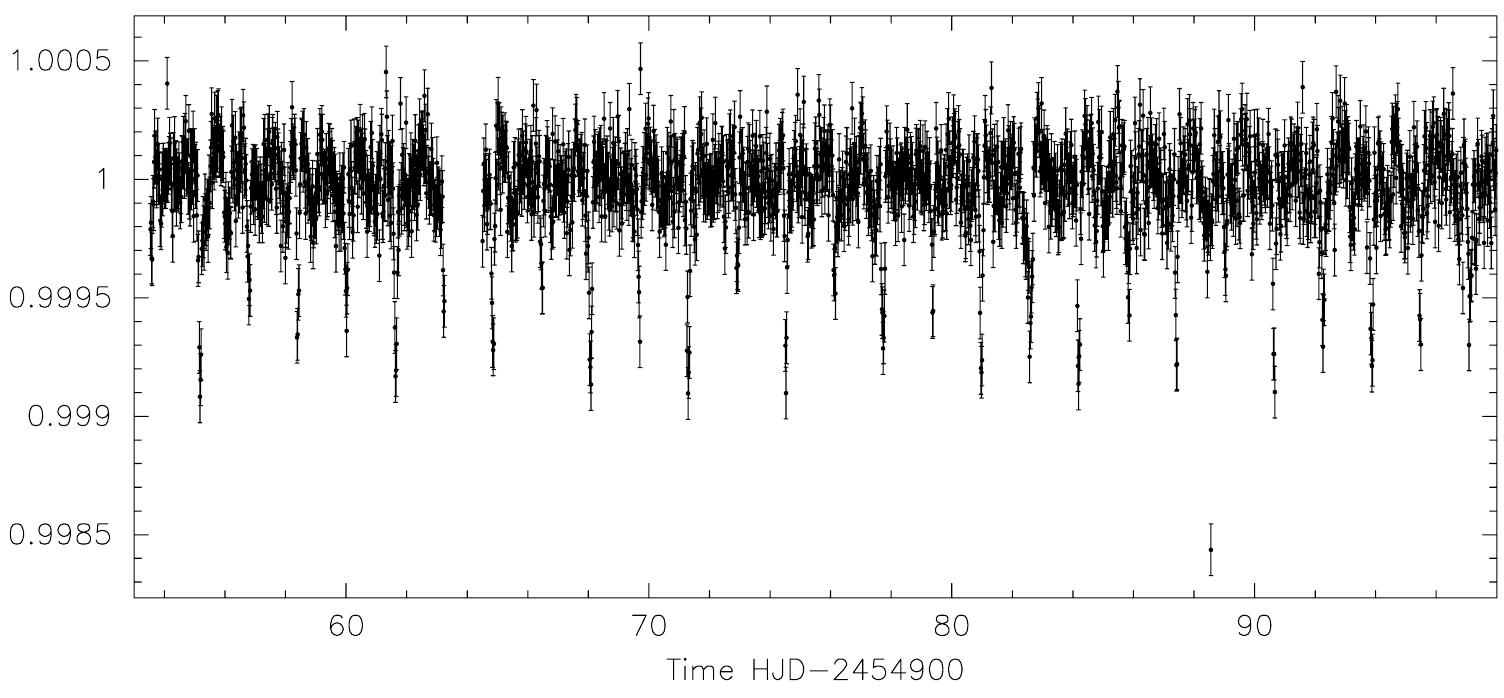
\includegraphics[width=1\textwidth]{keplertimeseries.png}
	\caption{\textbf{Kepler}: Detrended light curve of KOI-106\cite{keplertimeseriessource}. Small dips are planetary transits.}
	\label{fig:keplertimeseries}
\end{figure}

As described above, Kepler was designed with the purpose of exoplanet \textit{detection} in mind. It was later established that measurements of exoplanet radii from Kepler data, were possible. The investigation of the systemic effects observed over longer periods, in Kepler data, was presented via measurements of the HAT-P-7 system in \cite{hatp7}. It was concluded that it is not feasible to expect a precision greater than $1\%$, in the measurement of exoplanet radii using Kepler data. As explained above, measurements of exoplanet radii are dependent on accurate and precise measurements of the transit depth. The accuracy of this measurement is dependent on the absolute measurement of the depth and may be disturbed by flux variations induced by movements of the light on the CCD, as outlined above. The accuracy of the measurement also depends on knowledge of the linearity curve. Without this, we cannot know the true absolute value. Now, the precision of the measurement is dependent on the precision of the measurement of the linearity curve. All of this means that, if there had been a full linearity curve available for each of the Kepler CCDs, measured to the desired precision, the data could be corrected, and the temporal variations observed in \cite{hatp7} could be eliminated. This is because the roll maneuver performed by the spacecraft every quarter positions the starlight on a different CCD entirely. Knowledge of the difference in the two linearity curves of these two CCDs would allow for a correction of this flux change that is not due to variations in the system. 

This work demonstrates that construction of the linearity curve may be performed with relative ease, and should hence be done every time a new CCD is to be flown in space.

It was concluded for Kepler that the pointing stability had to be better than $0.003$ arcsec  $/15$ min \cite{keplermissionreq}. Direct comparison with results obtained above, tabulated in \ref{table:pointingresults}, depends on knowledge of the STEP optics. It was also demonstrated that this precision could be achieved without a shutter, which is also the case for the Atik 414EX detector. 

The Kepler mission applies a calibration pipeline to the data \cite{keplerpipeline}. This pipeline is akin to the corrections described in section \ref{sect:cal}. First, the image data is bias-corrected. Then it is adjusted for gain and nonlinearity. Lastly, it is corrected for hot pixels, cosmic rays, and dark current effects, and then flat-field corrected. The dataset is then detrended for jitter noise, pointing drifting and thermal transients are removed \cite{keplerpipeline}. This process can be seen in figure \ref{fig:keplerpdc}. The top curves in both panels clearly illustrate the importance of pointing precision. After calibration and preprocessing, Kepler produces time series data as seen in figure \ref{fig:keplertimeseries}.

\begin{figure}
	\centering
	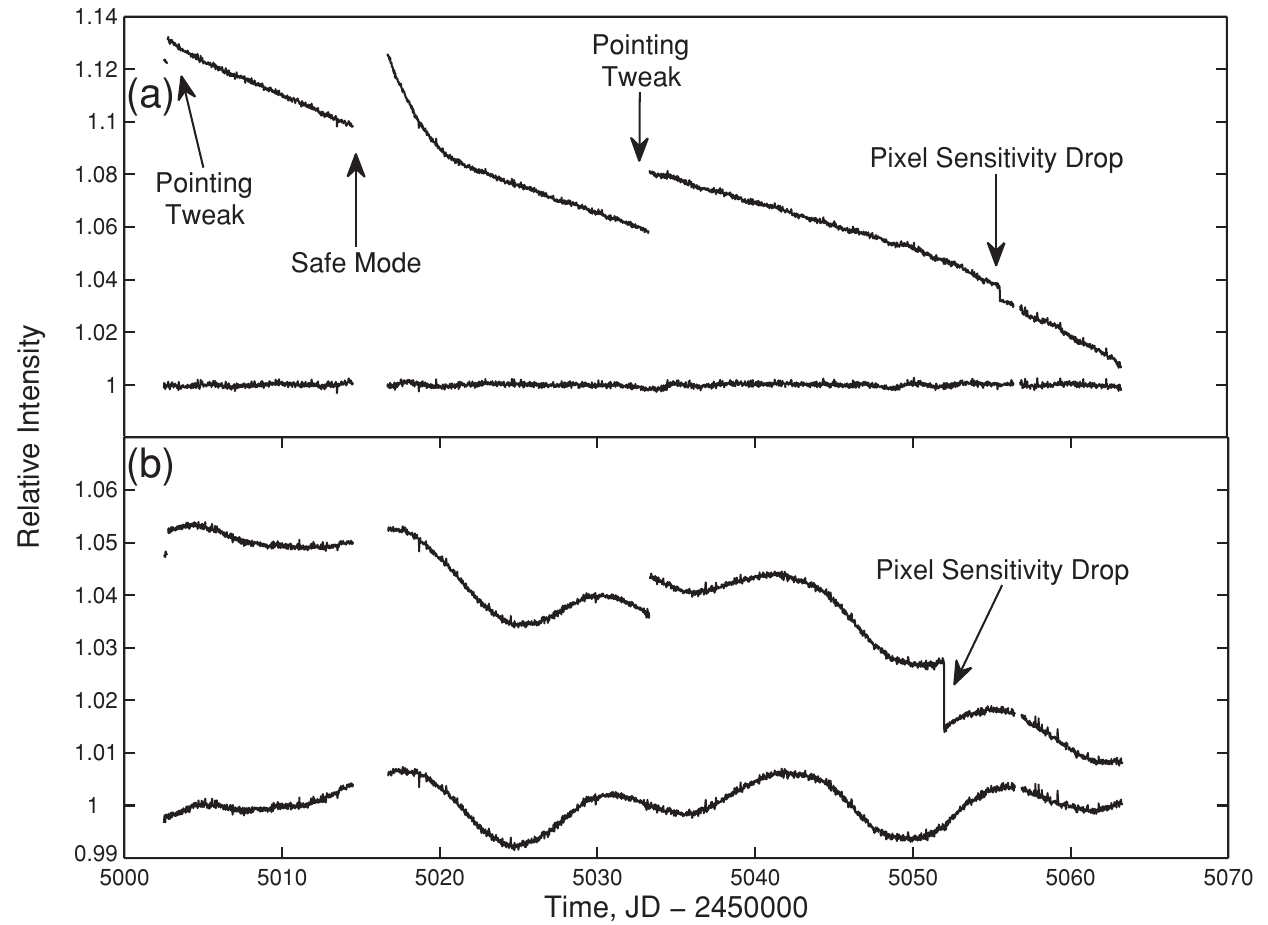
\includegraphics[width=1\textwidth]{pdckepler.png}
	\caption{\textbf{Kepler}: The raw and corrected data\cite{keplerpipeline}, after it has been detrended for jitter noise, pointing drifting and thermal transients. Top curves in each panel is the raw data, while the bottom curve is the detrended data set. }
	\label{fig:keplerpdc}
\end{figure}

\subsection{TESS}
\textbf{T}ransiting \textbf{E}xoplanet \textbf{S}urvey \textbf{S}atellite (\textbf{TESS}) is a space telescope in the NASA explorer program, and like Kepler carries CCDs as the main scientific instrumentation. TESS carries four cameras, each having a focal plane of four CCDs. The CCDs used are MIT/LL CCID-80 detectors. They are back-illuminated and fabricated at MIT Lincoln
Laboratory \cite{tesscharacterization}. The CCDs are of the frame transfer type. The entire image is rapidly parallel row transferred into the framed area, which is shielded from incoming starlight. A thorough characterization of the CCDs was carried out in \cite{tesscharacterization}. 

The characterization procedure was performed on a flight-grade engineering CCD. From this arises several concerns, as the characterization was not performed on the individual CCDs that were to be flown on the mission. One can argue that the expected deviation between the CCDs fabricated to the same standard, should be low, but at the same time, an argument can be made for the opposing viewpoint: We cannot in general be sure that the 16 CCDs are identical, and ideally, each of the CCDs that are to be flown on the mission should be characterized on the ground before flight, if practically feasible. 

The light source used in the characterization procedure was a fiber-coupled LED, diffused using an integrating sphere \footnote{An integrating sphere is a hollow sphere, where the inside walls of the cavity are painted with a diffusing white reflective coating. As light is incident from one side, it is diffused and scattered inside the sphere, eliminating any spatial and directional dependence of the light.}. Thus, the setup consists of a well-calibrated light source, that may uniformly illuminate the CCD chip. 

Transferring of charge into the shielded region takes  $19.95$ ms\cite{tessinstrumenthandbook}. Afterward, the CCD charge may be read out as slowly as is deemed necessary. Using this kind of readout process, in comparison to a rapid readout as was the case for Kepler, is evident in the much lower readout noise measured for the TESS CCDs. Read noise was measured to be in the range of $7-11 \;e^-$, which is of the same order of magnitude as that presented for the Atik 414EX detector in this work. 

\begin{figure}
	\centering
	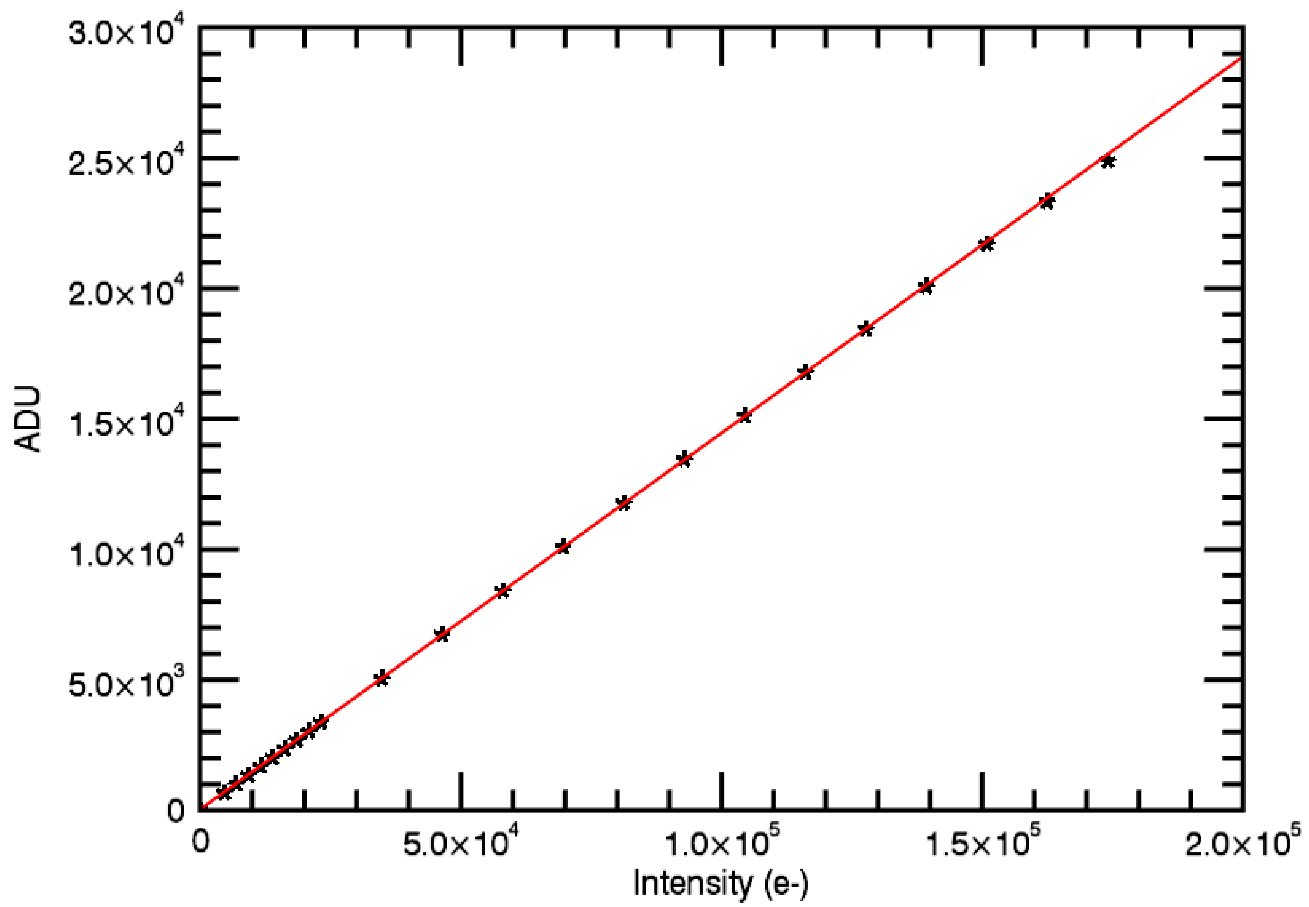
\includegraphics[width=0.85\textwidth]{tesslinearity.png}
	\caption{\textbf{TESS}: 	The measured ADU level as a function of the input intensity \cite{tesscharacterization}. The red line is a linear fit to the data set.}
	\label{fig:tesslinearity}
\end{figure}

Linearity was measured in a different manner than the method presented in this work. Instead of varying exposure times of the detector, the light source intensity was varied. Both of these methods will produce different levels of measured ADU as the main parameter (be it exposure time, or the intensity/flux level) is varied. This is predicated on access to a light source that may be varied predictably. Calibrating light sources to output a certain flux is not a simple task. Uncertainties in the knowledge of the actual flux level will impact the results obtained for the linearity curve. Varying the flux level is not necessary with the experimental procedure that has been presented in this work. Here it is the calibration of the time-keeping of the detector that is in question, and a procedure to determine the accuracy of this has been presented above as well. The linearity data obtained for the flight-grade characterization CCD in the case of TESS may be seen in figure \ref{fig:tesslinearity}. The deviation of the individual data points, from the fitted linear relation, may be seen in figure \ref{fig:tesslinearitydev}, which corresponds to figure \ref{fig:linearitydim} for the Atik 414EX detector.

\begin{figure}
	\centering
	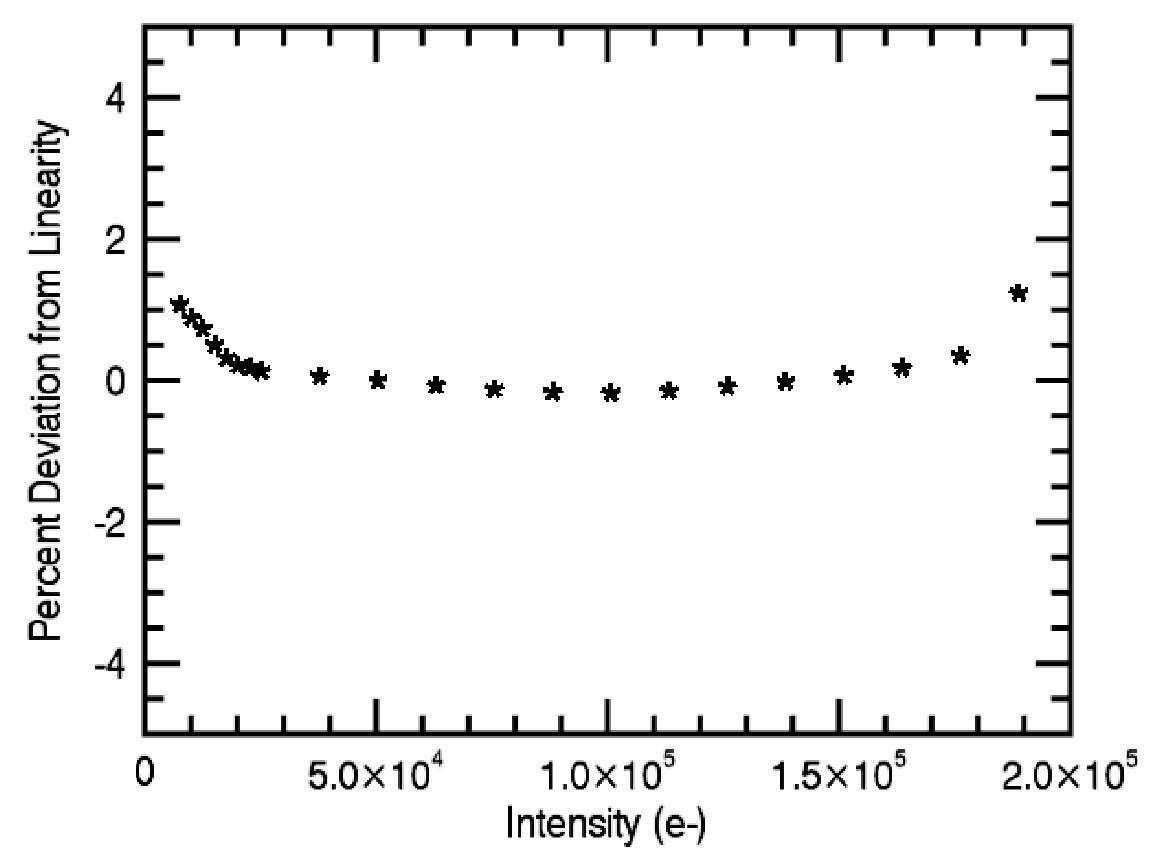
\includegraphics[width=.65\textwidth]{tesslinearitydev.png}
	\caption{\textbf{TESS}: The percentage deviation in the data points from the linear relation fitted, as a function of the input intensity \cite{tesscharacterization}.}
	\label{fig:tesslinearitydev}
\end{figure}

In comparison with the Kepler mission, linearity calibration data is present for the TESS mission, tabulated in the appendix of \cite{tessinstrumenthandbook}. The CCD was found to be linear to within $0.3\%$ deviation for most of the dynamic range\cite{tesscharacterization}, see figure \ref{fig:tesslinearitydev}. No reference to the precision of the measurement is given.

\subsection{CoRoT}
\begin{figure}
	\centering
	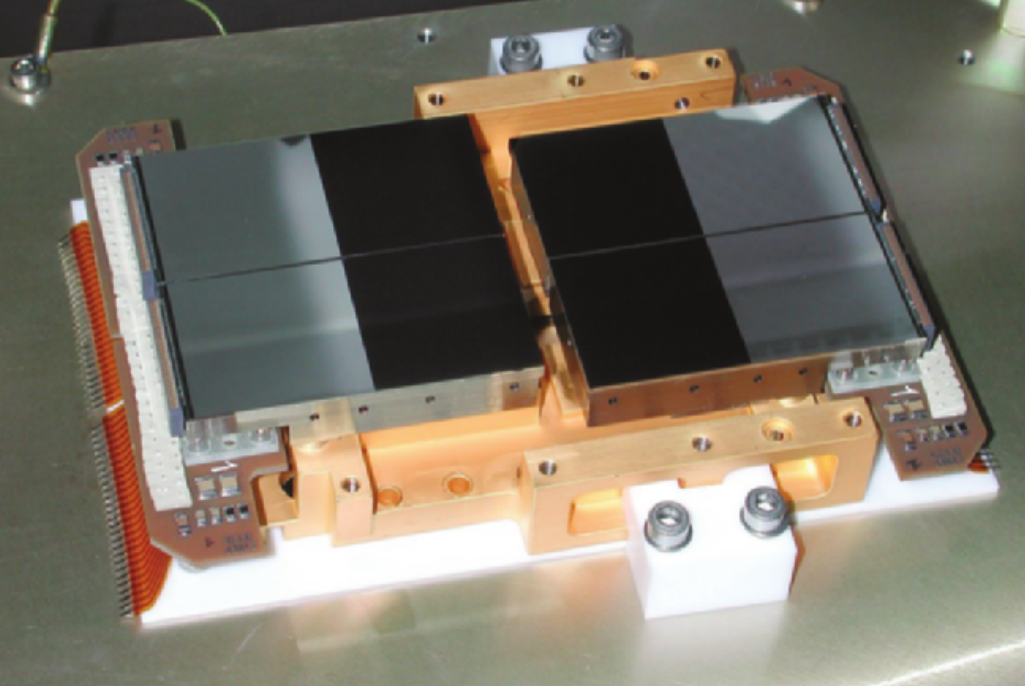
\includegraphics[width=0.7\textwidth]{corotfocalarray.png}
	\caption{The CoRoT focal plane, with the four frame transfer CCDs.}
	\label{fig:corotfocalplane}
\end{figure}
\textbf{Co}nvection, \textbf{Ro}tation et \textbf{T}ransits planétaires (Convection, Rotation and planetary Transits, \textbf{CoRoT}) was a french led (\textbf{CNES}) space telescope operated from 2006 to 2013, designed to search for large earth sized exoplanets of short orbital periods, and to perform asteroseismology.

The CoRoT focal plane consists of four frame-transfer, thinned, radiation protected, back-illuminated CCD detectors \cite{refId0}, that may be seen in figure \ref{fig:corotfocalplane}. In the characterization of the CCDs, described in \cite{corotCharCCD}, 9 similarly fabricated CCDs of the CoRoT specifications were characterized, and the four best were chosen. During characterization, the CCDs were cryogenically cooled. Cryogenically cooling the detectors is justified, as the same performance may be achieved in space by the use of radiators pointed into deep space. In comparison to the characterization of the TESS mission CCD, the CoRoT characterization was performed on the CCDs that were to be flown in space.

\begin{figure}
	\centering
	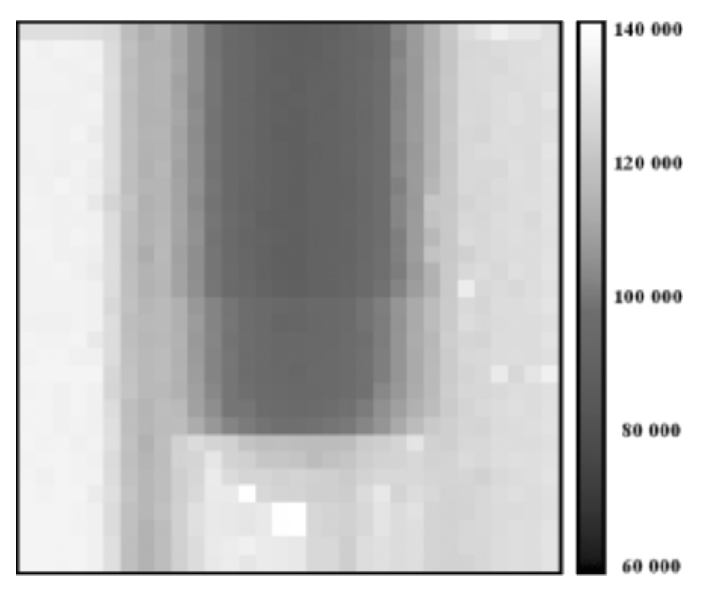
\includegraphics[width=0.7\textwidth]{corotprnu.png}
	\caption{A map of the measured pixel capacity of the CCD pixels, for one of the CCDs characterized for the CoRoT mission. Here, a significantly lower capacity is observed in the middle of the chip.}
	\label{fig:corotccdprnu}
\end{figure}

The light source(s) used were LEDs of different colors, using an integrating sphere, such as in the TESS CCD characterization. Dark current, gain, pixel capacity, Pixel Response Non-Uniformity (PRNU), and CCD temperature sensitivity were all measured. The latter has not been treated in this work, and will hence not be discussed, and the PRNU is akin to the flat field. 

Readout noise was measured in \cite{corotCharCCD2} to be $11 e^- $.
The characterization procedure used $30$ consecutively acquired frames summed to reduce photon and readout noise. Pixel capacity is found to be significantly lower in the center and top of 5 of the CCDs which proves to be the main limitation of the instruments, see figure \ref{fig:corotccdprnu}. This places a limit on exposure times, as the CCD will saturate earlier. Linearity was not measured.

Light spots on the satellite focal plane were defocused. The CoRoT focal plane is divided into two sections, one dedicated to Asteroseismology, and one to planet-finding. In front of the latter, a prism is situated, dispersing the light and providing a spectrum. This disperses light more strongly in the blue wavelength range \cite{refId0}. This results in a smeared-out point spread function (PSF) that is stronger in the blue light. Onboard processing applies an RGB mask to the PSF, which is essentially three areas of the PSF (dividing the spectrum into three areas), divided by hard cutoffs. Thus three new PSFs are constructed, one for the blue, green, and red light.
Naturally, issues arise from this. The first consideration is that say, the red RSF has a hard discontinuity. This means that any small movements of the PSF may cause a significant change in the flux measured, making photometry harder to do precisely. In addition, field crowding introduces effects that can be hard to correct for, and the result was that the RGB areas were summed to white light instead. Essentially the system sensitivity to movements was practically maximized. 

% Please add the following required packages to your document preamble:
% \usepackage[table,xcdraw]{xcolor}
% If you use beamer only pass "xcolor=table" option, i.e. \documentclass[xcolor=table]{beamer}
\begin{table}[]
	\centering
	\begin{tabular}{|l|l|l|l|l|}
		\hline
		\rowcolor[HTML]{C0C0C0} 
		{\color[HTML]{000000} \textbf{\begin{tabular}[c]{@{}l@{}}CCDs /\\ Measured values\end{tabular}}} & {\color[HTML]{000000} \textbf{\begin{tabular}[c]{@{}l@{}}Test procedure\\ detector\end{tabular}}} & {\color[HTML]{000000} \textbf{Kepler}} & {\color[HTML]{000000} \textbf{TESS}} & {\color[HTML]{000000} \textbf{CoRoT}} \\ \hline
		\cellcolor[HTML]{C0C0C0}{\color[HTML]{000000} \textbf{Readout noise}} & {\color[HTML]{000000} $3.2 - 12\;e^-$} & {\color[HTML]{000000} $81-307\;e^-$} & {\color[HTML]{000000} $7-11\;e^-$} & {\color[HTML]{000000} $11\;e^-$} \\ \hline
		\cellcolor[HTML]{C0C0C0}{\color[HTML]{000000} \textbf{Nonlinearity}} & {\color[HTML]{000000} $<3\%$} & {\color[HTML]{000000} $<3\%$} & {\color[HTML]{000000} $<0.3\%$} & {\color[HTML]{000000} $\text{N/A}$} \\ \hline
		\cellcolor[HTML]{C0C0C0}{\color[HTML]{000000} \textbf{Light Source}} & {\color[HTML]{000000} \begin{tabular}[c]{@{}l@{}}Diffuse reflection \\ of ambient room \\ light\end{tabular}} & {\color[HTML]{000000} N/A} & {\color[HTML]{000000} \begin{tabular}[c]{@{}l@{}}Integrating \\ sphere, fiber \\ coupled LED\end{tabular}} & {\color[HTML]{000000} \begin{tabular}[c]{@{}l@{}}Integrating\\ sphere, colored \\ LEDs\end{tabular}} \\ \hline
	\end{tabular}
	\caption{A tabularized summary of the comparison given in the discussion.}
	\label{table:missioncomp}
\end{table}

\subsection{MOST}
The Microvariablity and Oscillations of Stars (MOST) satellite mission, is Canada's first microsatellite science mission\cite{mostdescription}. It is an example of a different and creative solution to the pointing problem posed when a satellite is to provide precise photometric data. 
The main scientific goal was the characterization of stellar oscillations in solar-like stars (asteroseismology). It carries a telescope with a focal array of a guidance CCD and a science CCD, both of the frame-transfer type \cite{mostdescription}. 
At the time it was infeasible to construct ADCS solutions for microsatellites that could realize the desired photometric performance to observe stellar oscillations\cite{mostdescription}, so to realize ultra-precise photometry an array of 6 $\times$ 6  microlenses covers part of the science CCD (see figure \ref{fig:mostfabryarray}). It has been shown that such a configuration increases photons detected and reduces noise due to CCD pixel-by-pixel response variations, subpixel variation problems, and jitter noise. Thus, the movements of the stars are corrected by the lens. 
This means that flux changes resulting from movements have been removed from the CCD, and onto the optics in the system. Changes in the flux may still be present as a function of this movement, but now the movement can no longer be seen. The problem may have been moved, but it is practically impossible to deduce how the changes in the flux relate to movements. The result was that this microlens array wasn't used for photometry.

\begin{figure}
	\centering
	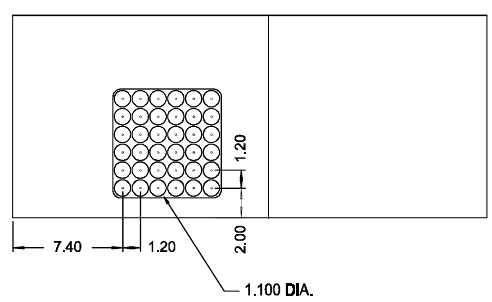
\includegraphics[width=0.7\textwidth]{mostfabryarray.png}
	\caption{A depiction of the $6\times 6$ array of microlenses covering prat of the (left) science CCD \cite{mostdescription}}
	\label{fig:mostfabryarray}
\end{figure}

\subsection{CHEOPS}
The CHaracterising ExOPlanet Satellite (CHEOPS) is the first small satellite mission in the ESA Science Programme \cite{cheopsmission}. It was launched on December 18, 2019, from Kourou, French Guiana. The mission is dedicated to observations of transits in systems already known to host planets\cite{cheopsmission}. The satellite carries a single thinned, frame-transfer, back-illuminated CCD. The main goal is the detection of Neptune-sized planets, with a photometric precision of $85$ ppm during a $3$ hour integration time, and Earth-sized planets with photometric precision of $20$ ppm, for a 6 hour integration time. It has a pointing accuracy of 1 arcsec. A requirement was that this stability is held for a minimum of 48 hours. 

To mitigate the issue of pointing jitter and drift, imperfect flat-fielding, sub-pixel response variations, and saturation in bright stars, CHEOPS is defocused on purpose. This naturally poses issues when observing crowded fields, and faint stars.

The flight CCD was characterized on a test bench using what the authors refer to as a "\textit{super stable lightsource}" of stability $3$ppm during $1$ minute \cite{cheopschar}. This light source is directed via a fiber to the focal plane, either as a point source or uniformly illuminating the CCD.

A readout noise of $14$ and $7 \; e^-$ was measured for a readout frequency of respectively $230$ and $100$ kHz\cite{cheopschar}, both comparable to the levels measured for both the test procedure and validation detectors in this work. The dark current was measured to an average value of $0.028 e^-/s$\cite{cheopschar}. Two hot pixels were identified, which is very good in comparison to those measured in this work. Nonlinearity in the dynamical range is quoted as less than $3\%$ as is the case for Kepler and CoRoT.

\subsection{Summary of comparisons and practical reccomendations}
The Kepler mission budget allowed for the construction of an expensive and well-calibrated setup for characterization, but the linearity calibration was not presented, resulting in systemic effects in the Kepler data. The TESS characterization was thorough but dependent on expensive well-calibrated equipment. Here, the calibration of the linearity curve was however dependent on the knowledge of the precision to which the light source intensity could be varied. For the CoRoT case, calibration data was lacking, and a prism poses significant issues concerning movements. The MOST mission illustrates the issues with attempting to move the problem of centroid movement, away from the CCD and onto other subcomponents. 

For all of these missions, where linearity was measured, it was done using highly calibrated light sources, varying intensities, and using integrating spheres. Flux changes resulting from movements have been attempted corrected by various optics. 

Common in all these approaches is that the experimental procedures seek to remove problems from the detector itself, either by controlling the light source, or the movement of the light. The present work serves to illustrate that this is not necessary at all. The choice of light source is not important, we can eliminate the effects by applying appropriate measurement schemes. Instead, we should simply calibrate the timekeeping of the detector. In addition, we should accept movements of the light centroid on the CCD. These effects cannot be eliminated, so it is better that the movement is on the detector, such that they may be tracked, and their relationship with the flux change may be deduced. This leads to a new and practical approach in which any physical effects that induce changes in the measured light, are kept at the detector. Thus, it may be concluded that:
\begin{quote}
	\textbf{\textit{Any effects that may disrupt the photometric performance, are entirely dependent on the detector in question, when using the approach specified in this work.}}
\end{quote}

\begin{tcolorbox}[colframe = white, sharpish corners]
	\textbf{Recommendation for future space missions}
	\begin{quote}
		Any CCD that is to be flown in space for use in astronomical photometric measurements, must be thoroughly characterized before launch. In space, the characterization must be verified. If the characterization has changed, the detector must be recharacterized.
	\end{quote}
\end{tcolorbox}

\section{Conclusion}
This work has studied the use of CCD detectors in astronomical satellite missions, with a focus on the Danish STEP mission. STEP aims to provide photometric observations of stars to measure exoplanet transits. Mission requirements were deduced from Kepler mission findings. These requirements are measurements of the CCD linearity curve to a precision of at least $5*10^{-4}$, and a maximum allowable flux change of $10^{-4}$ during observation of a transit. A CCD characterization procedure enables the first requirement to be met and has been presented above.

\begin{tcolorbox}[colframe = white, sharpish corners]
	\begin{quote}
		\textbf{A characterization procedure for CCDs that are to be used for photometry, has been developed and validated.}
	\end{quote}
\end{tcolorbox}

\noindent Following this procedure requires simple, inexpensive equipment, readily available in most university teaching labs. This procedure characterizes the bias, flat-field, gain, and noise levels of the detector, and enables full construction of the nonlinearity curve. A procedure to construct a time calibration of the detector enables the usage of an arbitrary light source. A measurement plan has been provided that takes temporal variations of the light source into account. It may be concluded that

\begin{tcolorbox}[colframe = white, sharpish corners]
	\begin{quote}
		\textbf{Any CCD may meet the photometric performance requirements if there is enough time to perform adequate repeat measurements of the nonlinearity curve. The characterization procedure and attitude test only depend on the CCD in question.}
	\end{quote}
\end{tcolorbox}

\noindent Any disruptions to the photometric performance of the mission are dependent on the choice of detector, and may hence be tracked and thus corrected if possible. Once the detector has been chosen, requirements on the photometric precision may be established. This precision may be met arbitrarily given enough repeat measurements of the linearity curve. This is not predicated on any particular, well-calibrated source of light. And the fact that it is possible to calibrate the nonlinearity of the detector, using any light source, is one of the main results of this work. 

\begin{tcolorbox}[colframe = white, sharpish corners]
	\begin{quote}
		\textbf{Construction of the nonlinearity curve of a CCD detector is not predicated on the usage of expensive experimental setups using finely calibrated light sources. It may be done using an ambient light source, such as a fluorescent light bulb in the ceiling, diffusively reflected off a white screen. Any temporal change in the flux intensity of the light source, that is linear between two adjacently acquired frames, can be corrected for, as described in the text.}
	\end{quote}
\end{tcolorbox}

\noindent Technical requirements to the ADCS subsystem can be output from scientific requirements, using the presented experimental procedure.

\begin{tcolorbox}[colframe = white, sharpish corners]
	\begin{quote}
		\textbf{An experiment to determine, with a given detector, the technical requirements for the ADCS subsystem, from the allowable flux change has been presented.}
	\end{quote} 
\end{tcolorbox}

\noindent This is also predicated on simple equipment, and once again, poses no constraints on the light source. As a result of this, given an arbitrary CCD, technical requirements to the ADCS subsystem can be output from scientific input requirements. The fact that these procedures and tests are simple and not predicated on highly calibrated equipment, means they can and should be done on a CCD that is to be flown in space. In addition, the test can be repeated in space, either as a recalibration or a validation.  \textbf{A recommendation for future space missions is}

\begin{tcolorbox}[colframe = white, sharpish corners]
	\begin{quote}
		\textbf{The above procedures and tests can (and should be) done any time a CCD is to be flown in space. The tests are repeatable in space, either as a validation, or a recalibration. }
	\end{quote} 
\end{tcolorbox}

\noindent This also opens the possibility of thorough characterization and testing of student-driven projects, without unnecessarily straining budgets. A comparison with other astronomical satellite missions has been given. Seasonal systemic variations are observed in the Kepler data set. The conclusion here is that such effects as those observed in the expensive Kepler instruments, could have been eliminated, by applying a simple calibration procedure such as the one presented here.
	
	
\end{document}